\documentclass[convert]{standalone}

\usepackage{tikz}
\pagestyle{empty}

% INT_AY22_L03_Fig08_y_ball_pos_vs_time.png

\begin{document}
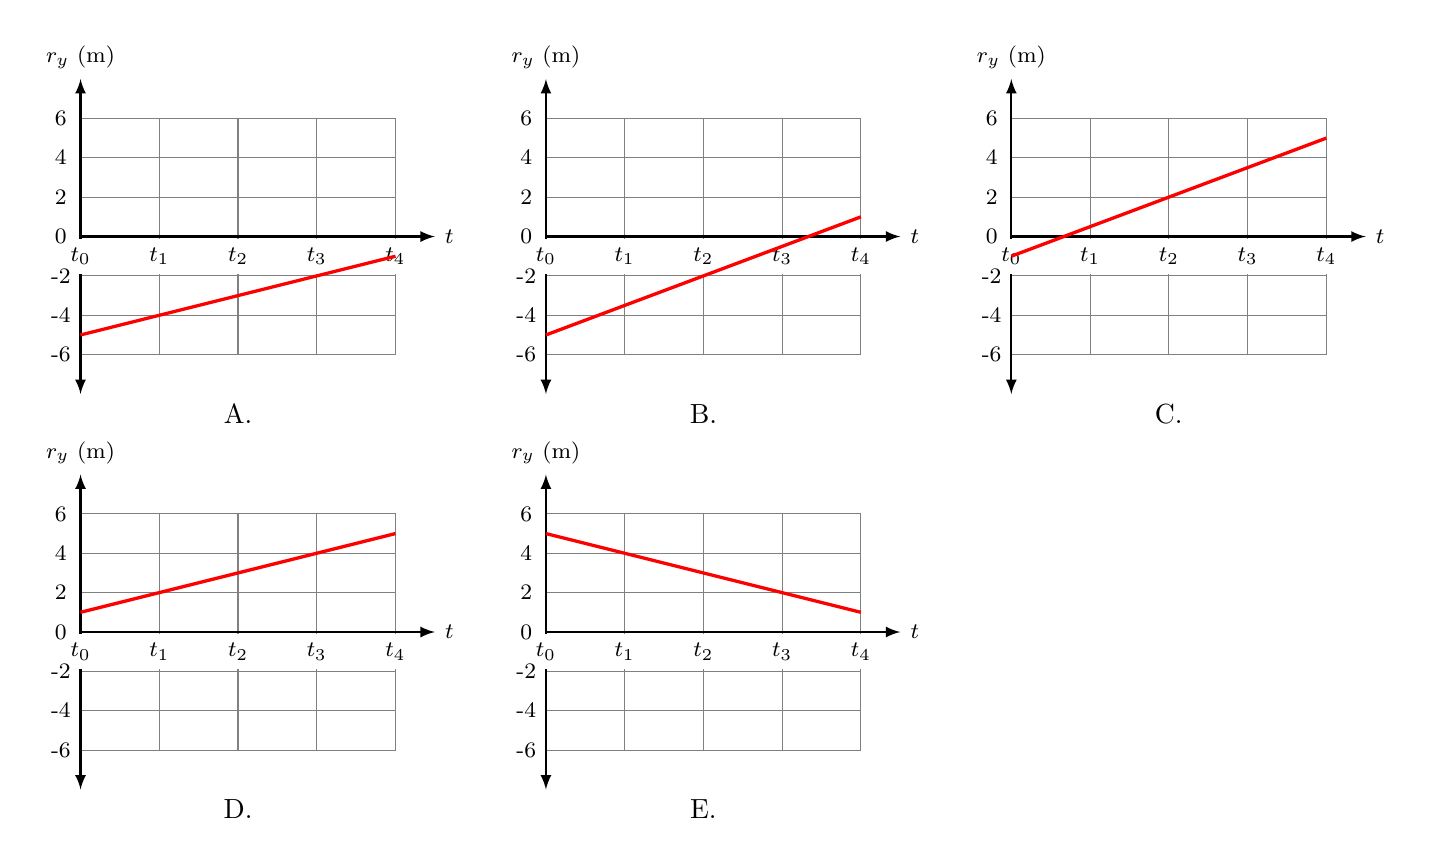
\begin{tikzpicture}[> = latex, font = \footnotesize]
\matrix[column sep = 0.5 cm]{

	% Definitions
	
	\def\xi{-2.5}		% Initial x, y coordinates
	\def\yi{2.5}
	
	\def\vx{1.5}		% Velocity components
	\def\vy{-0.5}
	
	% Draw graph grid
	
	\draw [thin, gray, xstep = 1 cm, ystep = 0.5 cm] (0, 0) grid (4, 3);
	
	% Draw axes + labels
	
	\draw [thick, <->] (0, 3.5) node [above] {$r_y$ (m)} -- (0, -0.5);
	\draw [thick, ->] (0, 1.5) -- (4.5, 1.5) node [right] {$t$};
	
	\foreach \x in {0, 1, 2, ..., 4}
		\node [fill = white] at (\x, 1.25) {$t_\x$};
	
	\foreach \y in {-6, -4, ..., 6}
		\node at (-0.25, 0.25 * \y + 1.5) {\y};
	
	% Draw curve
	
	\draw [very thick, red] (0, 0.25) -- (4, 1.25);
	
	% Graph label
	
	\node [font = \normalsize] at (2, -0.75) {A.};
	
&

	% Definitions
	
	\def\xi{-2.5}		% Initial x, y coordinates
	\def\yi{2.5}
	
	\def\vx{1.5}		% Velocity components
	\def\vy{-0.5}
	
	% Draw graph grid
	
	\draw [thin, gray, xstep = 1 cm, ystep = 0.5 cm] (0, 0) grid (4, 3);
	
	% Draw axes + labels
	
	\draw [thick, <->] (0, 3.5) node [above] {$r_y$ (m)} -- (0, -0.5);
	\draw [thick, ->] (0, 1.5) -- (4.5, 1.5) node [right] {$t$};
	
	\foreach \x in {0, 1, 2, ..., 4}
		\node [fill = white] at (\x, 1.25) {$t_\x$};
	
	\foreach \y in {-6, -4, ..., 6}
		\node at (-0.25, 0.25 * \y + 1.5) {\y};
	
	% Draw curve
	
	\draw [very thick, red] (0, 0.25) -- (4, 1.75);
	
	% Graph label
	
	\node [font = \normalsize] at (2, -0.75) {B.};
	
&

	% Definitions
	
	\def\xi{-2.5}		% Initial x, y coordinates
	\def\yi{2.5}
	
	\def\vx{1.5}		% Velocity components
	\def\vy{-0.5}
	
	% Draw graph grid
	
	\draw [thin, gray, xstep = 1 cm, ystep = 0.5 cm] (0, 0) grid (4, 3);
	
	% Draw axes + labels
	
	\draw [thick, <->] (0, 3.5) node [above] {$r_y$ (m)} -- (0, -0.5);
	\draw [thick, ->] (0, 1.5) -- (4.5, 1.5) node [right] {$t$};
	
	\foreach \x in {0, 1, 2, ..., 4}
		\node [fill = white] at (\x, 1.25) {$t_\x$};
	
	\foreach \y in {-6, -4, ..., 6}
		\node at (-0.25, 0.25 * \y + 1.5) {\y};
	
	% Draw curve
	
	\draw [very thick, red] (0, 1.25) -- (4, 2.75);
	
	% Graph label
	
	\node [font = \normalsize] at (2, -0.75) {C.};
	
\\

	% Definitions
	
	\def\xi{-2.5}		% Initial x, y coordinates
	\def\yi{2.5}
	
	\def\vx{1.5}		% Velocity components
	\def\vy{-0.5}
	
	% Draw graph grid
	
	\draw [thin, gray, xstep = 1 cm, ystep = 0.5 cm] (0, 0) grid (4, 3);
	
	% Draw axes + labels
	
	\draw [thick, <->] (0, 3.5) node [above] {$r_y$ (m)} -- (0, -0.5);
	\draw [thick, ->] (0, 1.5) -- (4.5, 1.5) node [right] {$t$};
	
	\foreach \x in {0, 1, 2, ..., 4}
		\node [fill = white] at (\x, 1.25) {$t_\x$};
	
	\foreach \y in {-6, -4, ..., 6}
		\node at (-0.25, 0.25 * \y + 1.5) {\y};
	
	% Draw curve
	
	\draw [very thick, red] (0, 1.75) -- (4, 2.75);
	
	% Graph label
	
	\node [font = \normalsize] at (2, -0.75) {D.};
	
&

	% Definitions
	
	\def\xi{-2.5}		% Initial x, y coordinates
	\def\yi{2.5}
	
	\def\vx{1.5}		% Velocity components
	\def\vy{-0.5}
	
	% Draw graph grid
	
	\draw [thin, gray, xstep = 1 cm, ystep = 0.5 cm] (0, 0) grid (4, 3);
	
	% Draw axes + labels
	
	\draw [thick, <->] (0, 3.5) node [above] {$r_y$ (m)} -- (0, -0.5);
	\draw [thick, ->] (0, 1.5) -- (4.5, 1.5) node [right] {$t$};
	
	\foreach \x in {0, 1, 2, ..., 4}
		\node [fill = white] at (\x, 1.25) {$t_\x$};
	
	\foreach \y in {-6, -4, ..., 6}
		\node at (-0.25, 0.25 * \y + 1.5) {\y};
	
	% Draw curve
	
	\draw [very thick, red] (0, 2.75) -- (4, 1.75);
	
	% Graph label
	
	\node [font = \normalsize] at (2, -0.75) {E.};
	
\\
};
	
\end{tikzpicture}
\end{document}